\chapter{Элементарная теория вероятностей}
\section{Вероятностная модель эксперимента с конечным числом исходов}
Пусть проводится некий эксперимент с \emph{конечным} количеством исходов,
которые мы обозначим через $ \omega_1, \dots, \omega_N $.

Эти исходы будем также называть \emph{элементарными событиями}, а их
совокупность  
\[
	\Omega = \{ \omega_1, \dots , \omega_N\}
\]
(конечным) \emph{пространством элементарных событий} или \emph{пространством
исходов}.
Нахождение $ \Omega $ есть первый шаг в построении \emph{вероятностной модели}.
\begin{example} 
	Однократное подбрасывание монетки даёт, очевидно, $ \Omega = \{\text{Г}, \text{Р}\} $.
	Пространство элементарных событий для эксперимента с подбрасыванием монетки
	$n$ раз будет состоять из $ N(\Omega) = 2^n$ событий, каждое из которых будет определяться
наборами из $n$ значений типа Г или Р:
\[
	\omega_i = (a_1, a_2, \dots , a_n), \quad \text{где } a_i = \{ \text{Г},
	\text{Р} \}.
\]
В данном случае можно провести биекцию между событиями и подмножествами множества из $ n $
элементов, если считать, что Г обозначает взятые в это подмножество элементы, а
Р --- не взятые.
\end{example}

В примере выше мы считали \emph{упорядоченные} различно комбинации различными.
Чтобы отличить набор, не уважающий порядок, вводится обозначение $
[a_1,\ldots,a_n] $.

Рассмотрим такой случай на примере изъятия шаров с последующим
\emph{возвращением}.
\begin{example}
	Будем считать, что количество шаров $ M $, а длина комбинации $ n $. Общее количество таких
	комбинаций будет равно $ N(\Omega) = M^n $. Ни выше, ни здесь мы данный вывод
	никак не обоснуем, однако это легко сделать, воспользовавшись начальными
	знаниями комбинаторики и индукцией.

	Рассмотрим случай, когда порядок внутри комбинации не объявляется. Очевидно,
	различных комбинаций $ N(\Omega) $ тогда будет меньше. Покажем, что для этого
	случая  
	\[
		N(\Omega) = C^n_{M+n-1},
	\]
	где $ C^l_k := k!/(l!(k-l)!) $ --- <<число сочетаний из $ k $ элементов по $ l
	$>>. Доказательство будем проводить через индукцию по $ n $. Примем за $ N(M,
n) $ интересующее нас число, то есть количество возможных комбинаций длины $n$
из $ M $
шаров. 

	Простейшему случаю $ n = 1 $ соответствует простейшее заключение $ N(M, 1) = M
	$, что подтверждает нашу гипотезу. Заметим ещё, что $ N(k, 1) = k $ и для
	любого $ k \leqslant M $.

	Будем считать, что утверждение доказано для $ n $ и докажем его для $ n + 1 $.
	Поскольку порядок отсутствует, будем считать, что элементы расположены, к
	примеру, по неубыванию. В общем случае выберем некоторый эталонный порядок и
	пронумеруем шары: $ a_1, a_2, \dots, a_M $. В случае с $ N(M, n+1) $, легко заметить, что
	рассматривая отдельно все комбинации, в которых первыми элементами будут $ a_1
	$, $a_2$ и так далее, мы будем получать соответственно количество возможных
	комбинаций $ N(M, n)$, $N(M-1, n)$, $ N(M-2, n) $ и так далее. При этом просуммировав все
	эти числа, мы, конечно, получим интересующее $ N(M,n+1) $. А сделать это
	легко, поскольку все числа до $N(M, n)$ включительно, благодаря индукции, нам
	уже известны.

	Таким образом, осталось лишь доказать важную и для дальнейшего изучения
	формулу биномиальных коэффициентов
	\begin{equation}
		\label{eq:bin_coef}
		C^{l-1}_k + C^l_k = C^l_{k+1},
	\end{equation}
на чём мы останавливаться не будем. Скажем лишь, что это свойство лежит в основе
составления \emph{треугольника Паскаля}. Кроме того,  его легко доказать, заметив,
что первое слагаемое есть число комбинаций без порядка, в которые не входит
некий шар $ a_0 $, а второе --- общее число комбинаций длиной $ k $. Эту формулу
можно также вывести в лоб. 

Действительно, воспользуемся формулой \eqref{eq:bin_coef} и получим \qed
%TODO: proof
\end{example}

Тот же факт можно доказать проще. Пусть есть одна из таких комбинаций (без
порядка, но с повторениями) длины $ n $ с $ m $ возможными категориями шаров.
Тогда её можно представить как набор из $ n + m - 1$ единиц и нулей,
где, скажем, единица разделяет категории шаров. Поскольку категорий $ m $, то
разделителей будет $ m-1 $, а самих шаров по-прежнему $ n $. В такой комбинации
уже важен порядок, но в ней есть и повторения. Теперь к тому же исходных
множеств два. Выберем вместо этого тогда не сами элементы, а места под них.
Будем ставить в соответствие некоторым из $ m+n-1 $ мест $ m - 1 $
разделителей-единиц. При этом места не могут повторяться, а порядок вновь не
важен. Получили инъекцию из $ m-1 $ разделителей в $ m+n-1 $ мест. Согласно
одному из свойств биномиальных коэффициентов,  
\[
	C^{m-1}_{m+n-1} = C^{(m+n-1)-(m-1)}_{m+n-1} = C^n_{m+n-1}
\]
Действительно, мы выбирали $ m-1 $ единиц, хотя могли выбирать $ n $ нулей.
\qed



Перечислим ещё некоторые \textbf{свойства биномиальных коэффициентов}:
% TODO: свойства биномиальных коэффициентов

\begin{figure}[h!]
	\centering
	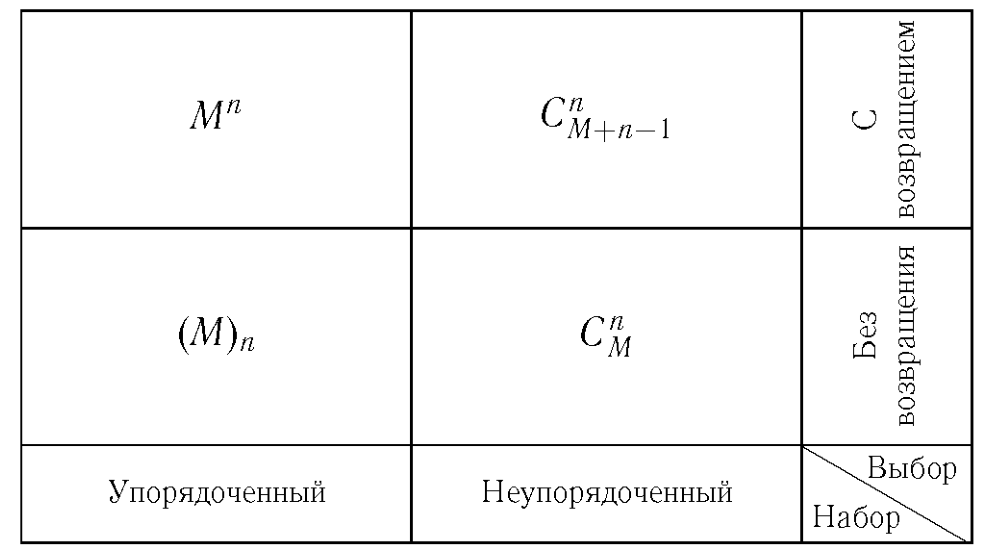
\includegraphics[width=0.8\textwidth]{Figures/table-1.png}
	\caption{Резюме}
	\label{fig:table-1}
\end{figure}


\subsection{Перестановки}
Перестановки без повторений $ n $ элементов осуществляются $ n! $ способами, это
легко проверить по индукции. 


\subsection{Ячейки и дробинки}
Выберем \emph{ячейки для дробинок}.
Пусть дробинки различимы. Тогда опыт описывается набором $ (a_1, \ldots, a_n) $.
Иначе --- набором $ [a_1, \ldots, a_n] $. Аналогично можно провести аналогию для
размещений с запретом (одна ячейка содержит не более одной дробинки) и без. В
первом случае имеем выбор с возвращением, во втором --- без. Имеем 
\begin{figure}[h!]
\begin{center}
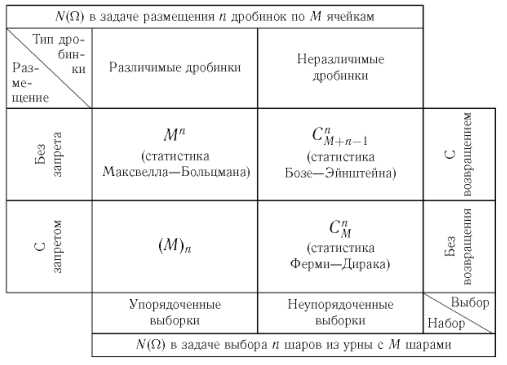
\includegraphics[width= \textwidth]{Figures/drob.png}
\end{center}
\label{fig:drob}
\end{figure}


\subsection{Событие}
\begin{definition}
	\emph{Событием} называем такое подмножество $ A \subset \Omega$ всех исходов,
	для которого по условиям эксперимента возможен однозначный ответ $ \omega \in
	A$ или $ \omega \notin A $. Событие $ \varnothing $ называем
	\emph{невозможным}, а $ \Omega $ --- достоверным.
\end{definition}

Объединение множеств $ A \cup B $ в том случае, когда они не пересекаются,
называется \emph{суммой} множеств и обозначается $ A + B $.

Система событий может образовать \emph{алгебру} $ \mathscr A $ с операциями $ \cup $, $ \cap $
и $ \setminus $, при условии $ \Omega \in \mathscr A $. Обычно берётся алгебра
всех подмножеств $ \Omega $.

\subsection{Вероятность}
Припишем каждому элементарному событию $ \omega_i \in \Omega $ некоторую
\emph{вероятность исхода},
обозначаемую $ p(\omega_i) = p_i $. Потребуем для этой величины выполнение
следующих условий: 
\begin{enumerate}
	\item $ 0 \leqslant p_i $,
	\item $\sum_{i=1}^N p_i = 1$ (\emph{нормированность}).
\end{enumerate}
Вероятность события тогда определим формулой 
\[
\mathsf P(A) = \sum_{\{i\colon\omega_i\in A\}} p_i.
\]
Перечислим некоторые \textbf{свойства вероятностей}: 
\begin{gather*}
		\mathsf P (\varnothing) = 0,\\
		\mathsf P (\Omega) = 1,\\
		\mathsf P (A \cup B) = \mathsf P(A) + \mathsf P(B) - \mathsf (A\cap B).
\end{gather*}


\begin{definition}
	Совокупность $ (\Omega, \mathsrc A, \mathsf P) $ называют \emph{вероятностным
	пространством}. Оно определяет \emph{вероятностною модель} эксперимента с
	конечным пространством исходов $ \Omega $ и алгеброй событий $ \mathsrc A $. 
\end{definition}



\section{Некоторые классические модели и распределения}
%TODO: section



\section{Условная вероятность}
%TODO: section



\section{Случайные процессы и их характеристики}
Заботят часто не столько элементарные события целиком, сколько лишь некоторые
числовые характеристики, зависящие от них (например, число решек в орлянке).

\begin{definition}
Всякая функция $ \xi(\omega) \in \mathbb R $, определённая на (конечном) $ \Omega $, будет
называться (простой) \emph{случайной величиной}.
\end{definition}

Обозначим (конечное) множество значений случайной величины $ \xi $ как $ X $, а
алгебру его подмножеств как $ \mathscr X $. Подмножество $ B \in \mathscr X $
можно интерпретировать как некоторое событие. Тогда	 
\[
	P_\xi (B) := \mathsf P\{\omega \colon \xi(\omega) \in B\}, \quad B \in \mathscr
	X. 
\]
\sloppy При этом ясно, что достаточно определить 
\[
	P_\xi(x_i) := \mathsf P \{\omega \colon \xi(\omega) = x_i\}, \quad x_i \in X
\]
вероятности прообраза каждого возможного значения.
Набор чисел $ \{ P_\xi(x_1), \ldots, P_\xi(x_m)\} $ называется
\emph{распределением вероятностей случайной величины $ \xi $}.

\begin{example}
	Случайная величина $ \xi $, принимающая значение 1 с вероятностью <<успеха>> и
	0 с вероятностью <<неуспеха>> называется \emph{бернуллиевской}. Для неё 
	\[
		P_\xi(x) = p^xq^{1-x}, \quad x=0,1.
	\]
	\emph{Биномиальной случайной величиной $ \xi $} называется случайная величина с вероятностями 
	\[
		P_\xi(x) = C^x_np^xq^{n-x}, \quad x = 0, 1, \ldots, n.
	\]
\end{example}

\begin{definition}
	Функция  
	\[
		F_\xi(x)=\mathsf P\{\omega\colon\xi(\omega)\leqslant x\}
	\]
	называется \emph{функцией распределения случайной величины $ \xi $}.
\end{definition}

Ясно, что 
\[
	F_\xi(x) = \sum_{\{i\colon x_i \leqslant x\}} P_\xi(x_i)
\]
и 
\[
		P_\xi(x_i) = F_\xi(x_i) - F_\xi(x_i-).
\]

Из определения вытекают следующие \textbf{свойства функции распределения}:
\begin{enumerate}
	\item $ F_\xi(-\infty) = 0 $, $ F_\xi(\infty) = 1 $;
	\item $ F_\xi(x+)=F_\xi(x) $.
\end{enumerate}

Иногда приходится рассматривать \emph{случайный вектор} $ \xi = (\xi_1, \ldots,
\xi_r)$, компоненты которого есть случайные величины. Например, в
мультиномиальном распределении. В этом случае набор вероятностей 
\[
		P_\xi(x_1, \ldots, x_r) = \mathsf P\{\omega\colon \xi_1(\omega) = x_1,
		\ldots, \xi_r(\omega)=x_r\},
\]
где $ x_i \in X_i $ --- области допустимых значений $ \xi_i $, называется
\emph{распределением вероятностей случайного вектора $ \xi $}, а функция 
\[
		F_\xi(x_1, \ldots, x_r) = \mathsf P\{\omega\colon \xi_1(\omega)\leqslant
		x_1, \ldots, \xi_r(\omega) \leqslant x_r\},
\]
$ x_i \in \mathbb R $, называется \emph{функцией распределения случайного
вектора $ \xi = (\xi_1, \ldots, \xi_r) $}.

Случайные величины $ \xi_1, \lsots, \xi_r $ называются \emph{независимыми}, если
для любых $ x_1\ldots,x_r\in X$ 
\[
	\mathsf P \{\xi_1 = x_1, \ldots, \xi_r = x_r\} = \mathsf
	P\{\xi_1=x_1\}\ldots\mathsf\{\xi_r=x_r\},
\]
или, что эквивалентно, для любых $ B_1,\ldots,B_r \in \mathscr X $ 
\[
	\mathsf P\{\xi_1\in B_1, \ldots, \xi_r\in B_r\} = \mathsf P\{\xi_1 \in
	B_1\}\ldots\mathsf P\{\xi_r\in B_r\}.
\]
Простейший пример независимых случайных величин можно получить, 
рассматривая схему Бернулли.

Важную роль играют функции от случайных величин, которые сами, конечно, являются
случайными величинами. Например, для $ \zeta := \eta
+ \xi$, $ z\in \mathbb R $ имеем  
\[
	P_\zeta(z) = \mathsf P\{\zeta = z\} = \mathsf P\{\xi +\eta = z\} =
	\sum_{\{(i,j)\colon x_i + y_j = z\}} \mathsf P\{\xi = x_i, \eta= y_j\}.
\]
Особенно важен случай независимых случайных величин $ \xi $ и $ \eta $. Там
\[
	\mathsf P\{\xi = x_i, \eta = y_i\} = \mathsf P\{\xi = x_i\} \mathsf
	P\{\eta=y_j\},
\]
и, значит,  
\[
	P_\zeta(z) = \sum_{\{(i,j)\colon x_i + y_j = z\}} P_\xi(x_i)P_\eta(y_j) =
	\sum_{i=1}^k P_\xi(x_i) P_\eta(z-x_i).
\]


\subsection{Характеристики случайных величин}
Сформулируем важнейшее понятие \emph{математического ожидания} случайных
величин. Обозначим $ p_i := \mathsf P\{\xi = x_i\} $. Интуитивно мы хотели
бы\footnote{Это предположение в дальнейшем получит в некотором смысле
подтверждение},
чтобы при наблюдении за значениями случайной величины $ \xi $ в <<$ n $
повторных независимых экспериментах>> при больших $ n $ значение $ x_i $
встретилось бы
примерно $ np_i $ раз. Тогда средним значением случайной величины будет равно
примерно 
\[
	\frac{1}{n} [np_1x_1 + \ldots + np_kx_k] = \sum_{i=1}^k p_ix_i.
\]
Это замечание делает понятным следующее 
\begin{definition}
\emph{Математическим ожиданием}, или \emph{средним значением} случайной величины
$ \xi = \sum_{i=1}^k x_i I(A_i) $ с множеством значений $ X = \{x_1, \ldots,
x_k\} $ называется число 
\[
	\mathsf E \xi = \sum_{i=1}^k x_i \mathsf P(A_i) = \sum_{i=1}^k x_i
	P_\xi(x_i) = \sum_{i=1}^k x_i \Delta F_\xi(x_i),
\]
где $ A_i := \{ \omega\colon \xi(\omega) = x_i\} $ --- прообраз значения $ x_i $, $ i =
\overline{1, \ldots, k} $; $ \Delta F_\xi(x) := F_\xi(x)-F_\xi(x-) $. Множества $ A_i $, естественно, образуют разбиение
множества $ \Omega $.
\end{definition}

Сформулируем основные \textbf{свойства математических ожиданий}:
\begin{enumerate} %[style=multiline,leftmargin=3cm,font=\textscfont]
	\item \textsc{Неотрицательность}. Если $ \xi \geqslant 0  $, то $ \mathsf E \xi
		\geqslant 0 $.
\item\textsc{Линейность.} $ \mathsf E(a\xi + b\eta) = a\mathsf E\xi + b \mathsf E\eta
		$.
	\item\textsc{Монотонность.} Если $ \xi \geqslant \eta $, то $ \mathsf E\xi \leqslant
		\mathsf E \eta$.
	\item \textsc{Неравенство треугольника.} $ |\mathsf E\xi| \leqslant \mathsf E
		|\xi|$.
	\item\label{enum:nez} Если $ \xi $ и $ \eta $ независимы, то $ \mathsf E \xi \eta = \mathsf E
		\xi \cdot \mathsf E\eta$.
\item\textsc{Неравенство Коши-Буняковского.} $ (\mathsf E
		|\xi\eta|)^2\leqslant\mathsf E \xi^2 \cdot \mathsf E\eta^2 $.
	\item Если $ \xi = I(A) $, то $ \mathsf E \xi = \mathsf P(A) $.
\end{enumerate}
Все свойства в сущности очевидны. \emph{Докажем}, например, второе.

Пусть  
\[
	\xi = \sum_{i} x_i I(A_i), \quad \eta = \sum_{j} y_i I(B_i).
\]
Тогда 
\[
	a\xi + b\eta = \sum_{i,j} (a\xi + b\eta) I(A_i\cap B_j),
\]
а 
\begin{multline*}
	\mathsf E(a\xi + b\eta) = \sum_{i,j} (ax_i + by_i) \mathsf P(A_i\cap B_j)=
	a\sum_i x_i \mathsf P(A_i) + b\sum_j y_j \mathsf P(B_j).
\end{multline*}
\qed

\begin{remark*} Свойство \ref{enum:nez} очевидным образом обобщается на любое
	конечное число случайных величин.
\end{remark*}





\section{Закон больших чисел}
